\documentclass[11pt,a4paper]{article}
\usepackage[flat]{pinns-course}

\coursemeta{Session 1, computational lab --- Universal approximation in numbers}{Session 1, computational lab}{universal approximation, random features, nonconvexity, PyTorch, M2 MACIA, AGM, CY Cergy Paris University}

% ================================================================
\begin{document}

\coursetitle{Session 1 \textbullet\ Computational lab}{Universal approximation, in numbers}{}

\vspace{6pt}

\begin{plainbox}
\textbf{What this is.} A short companion to the problem class \emph{Session 1 $\cdot$ Universal
approximation}. Four tasks, each reproducing numerically a statement you proved on paper, and one
--- Task \ref{task:gap} --- showing something the paper cannot show.

\smallskip
\textbf{Material.} Two notebooks, \code{lab1-student.ipynb} (with gaps) and
\code{lab1-solutions.ipynb}. Python with \code{torch}, \code{numpy}, \code{matplotlib}; no GPU, no
dataset, nothing to download. Every experiment runs in under a minute on a laptop.

\smallskip
\textbf{A note on using PyTorch now.} You will call \code{torch.autograd.grad} in Task
\ref{task:ridge} and \code{torch.optim.Adam} in Task \ref{task:gap}, two weeks before Session 2
explains what they do. That is deliberate and it is the only place in this course where a black box
is acceptable: here they are instruments, and what we measure with them does not depend on knowing
their internals. Session 2 opens both boxes and proves what is in them.
\end{plainbox}

\vspace{4pt}

\begin{warnbox}
\textbf{The rule of this lab.} \emph{Predict before you run.} Each task asks for a prediction first.
A computation that confirms what you already proved teaches you nothing; a computation that
contradicts what you expected teaches you a great deal. Task \ref{task:gap} is designed to
contradict a reasonable expectation.
\end{warnbox}

% ================================================================
\section{Task 1 --- Slabs, not bumps}

\begin{plainbox}
\textbf{Recalls.} A one-hidden-layer network is
$\Phi_\theta(x) = \sum_{i=1}^n c_i\,\sigma(w_i\cdot x + b_i)$. In Exercise 1 of the problem class you
showed that for sigmoidal $\sigma$ and $a<b$,
\[
\sigma\big(\lambda(x-a)\big) - \sigma\big(\lambda(x-b)\big) \xrightarrow[\lambda\to\infty]{} \ind_{(a,b)}
\]
pointwise off $\{a,b\}$ --- a \emph{bump} built from two neurons in dimension one --- and you argued
that the construction does not transpose to $d\ge2$. Proposition 1.5 of the lecture notes made the
obstruction precise: if $f \in \Sigma_1(\sigma)$ then $\nabla f(x)$ is collinear to a fixed vector
$w$ \emph{for every} $x$, and this fails for $\tfrac12(f_1+f_2)$.
\end{plainbox}

\begin{task}[What a ridge function looks like]\label{task:ridge} \tagcore
\leavevmode
\begin{enumerate}[label=\textbf{\arabic*.}]
\item Plot the bump of Exercise 1 for $\lambda = 2, 10, 100$. Nothing to predict here; this is to
have the object in front of you.
\item On $[-2,2]^2$, draw the level sets of $\sigma(w_1\cdot x)$, of $\sigma(w_2\cdot x)$ with
$w_1 = e_1$, $w_2 = e_2$, and of $\tfrac12(f_1+f_2)$. \emph{Predict the shape of each set of level
curves before plotting.}
\item Now measure Proposition 1.5. Sample $4000$ points at random, compute $\nabla f$ with
\code{torch.autograd.grad}, normalise each gradient, and report the \emph{angular spread} of the
directions, $\max\theta - \min\theta$. Do it for a single ridge function and for the half-sum.
\emph{Predict both numbers before running.}
\item Explain the first number. It is not small --- it is exactly zero, in double precision. Why
could it not have been anything else?
\end{enumerate}
\end{task}

\begin{figure}[h]
\centering
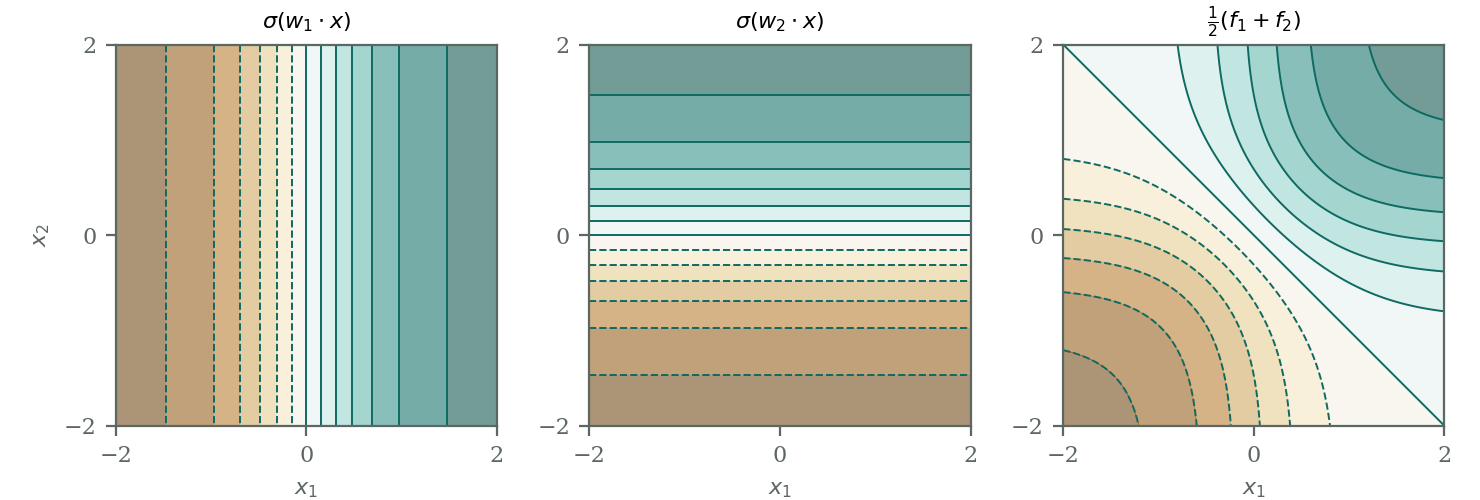
\includegraphics[width=\textwidth]{figures/fig_ridge2d.png}
\vspace{-4pt}
\caption*{\small\color{coursgrey} What you should obtain in Task \ref{task:ridge}, item 2. Straight
parallel level sets on the left and in the middle --- each ridge function is constant on every
hyperplane orthogonal to its own $w$, a \emph{slab} --- and curved level sets on the right. The
curvature is the geometric content of Proposition 1.5.}
\end{figure}

% ================================================================
\section{Task 2 --- A cap that width cannot lift, and depth can}

\begin{plainbox}
\textbf{Recalls.} In Exercise 2 you proved that with $\sigma(t)=t^2$ and \emph{fixed} depth $L$, the
realised function is a polynomial of degree at most $2^{L-1}$, whatever the width; and that letting
$L$ grow recovers every polynomial, via $xy = \tfrac14\big((x+y)^2-(x-y)^2\big)$.
\end{plainbox}

\begin{task}[The degree bound is attained]\label{task:poly} \tagcore
\leavevmode
\begin{enumerate}[label=\textbf{\arabic*.}]
\item Take a network with activation $t^2$, depth $L$ and \emph{random} weights --- no training.
Sample it on $400$ points of $[-1,1]$ and fit a polynomial of degree $2^{L-1}$, then of degree
$2^{L-1}-1$. \emph{Predict the two residuals} for $L=2,3,4$, then run.
\item Why does this experiment need no optimisation at all? Say in one sentence what that tells you
about the kind of statement Exercise 2 is.
\item Look at the residual one degree \emph{below} the bound, for $L=2,3,4$: it is roughly
$10^{-1}$, $10^{-2}$, $10^{-3}$. Comment. Which distinction, central to this course, does that
decreasing sequence illustrate?
\end{enumerate}
\end{task}

% ================================================================
\section{Task 3 --- The loss is not convex, drawn}

\begin{plainbox}
\textbf{Recalls.} Exercise 2.4 of the lecture notes: for the target $f = \tanh$ on $\Omega=(-1,1)$,
the parameters $\theta_+ = (c,w,b) = (1,1,0)$ and $\theta_-=(-1,-1,0)$ both realise $\tanh$, because
$\tanh$ is odd. Hence $J(\theta_+) = J(\theta_-) = 0$, while the midpoint $(0,0,0)$ realises the
zero function.
\end{plainbox}

\begin{task}[One picture, one proof]\label{task:nonconvex} \tagcore
\leavevmode
\begin{enumerate}[label=\textbf{\arabic*.}]
\item Plot $t \mapsto J\big((1-t)\theta_+ + t\,\theta_-\big)$ for $t \in [0,1]$.
\item \emph{Before running:} predict the value at $t = \tfrac12$, in closed form.
\item The curve exceeds the larger of its endpoint values. State, in one sentence, the property of
the \emph{parametrisation} --- not of the activation, not of the target --- that produces this.
\item A colleague proposes: ``the loss is nonconvex because the class of functions is nonconvex''.
Why is that not a proof? \emph{(Recall the counterexample of Exercise 2.4: composing a convex
functional with a nonaffine map can perfectly well be convex.)}
\end{enumerate}
\end{task}

% ================================================================
\section{Task 4 --- Existence is not an algorithm}

\begin{plainbox}
\textbf{The idea.} Cybenko's theorem asserts that a good $\theta$ \emph{exists}. To separate
existence from finding, freeze the inner parameters:

\smallskip
If $(w_i,b_i)$ are drawn at random and held fixed, then $\Phi_\theta$ depends \emph{linearly} on the
outer coefficients $c$, so $\min_c J$ is a linear least-squares problem --- convex, with a closed-form
solution obtained by \code{torch.linalg.lstsq}. Whatever error it achieves is therefore achieved by
an element of $\Sigma_n(\sigma)$ that we can exhibit. It is an upper bound on the best possible error
over $\Sigma_n(\sigma)$, obtained with no optimisation difficulty whatsoever.

\smallskip
Then train \emph{all} the parameters --- $c$, and the $(w_i,b_i)$ too --- with a gradient method, at
the same $n$. Training searches a strictly \emph{larger} set, so one might expect it to do at least
as well.
\end{plainbox}

\begin{task}[$\Ee_{\mathrm{app}}$ against $\Ee_{\mathrm{opt}}$]\label{task:gap} \tagcore
Target: $f(x) = \sin(2\pi x) + \tfrac14\sin(16\pi x)$ on $[0,1]$, one slow mode and one fast.
\begin{enumerate}[label=\textbf{\arabic*.}]
\item \emph{Predict, and write your prediction down before running:} for $n$ from $8$ to $256$, which
of the two procedures gives the smaller error, and by roughly how much?
\item Implement both and tabulate the RMS error for $n = 8, 16, 32, 64, 128, 256$. Plot on a
log--log scale.
\item Account for the behaviour at small $n$, where training wins. Why is that not a paradox?
\item Account for the behaviour at large $n$. Both numbers concern the \emph{same} class
$\Sigma_n(\tanh)$. What exactly has been demonstrated about the existence of a good network, and
about the ability of the method to find one?
\item Name the two error terms you have just separated, and say which later session is devoted to
each.
\item \emph{Push back on the experiment.} It uses one optimiser, one learning rate, one budget of
$4000$ steps. Change one of them --- more steps, a schedule, or \code{torch.optim.LBFGS} --- and
report what moves and what does not. What part of the conclusion survives your best effort?
\end{enumerate}
\end{task}

\begin{figure}[h]
\centering
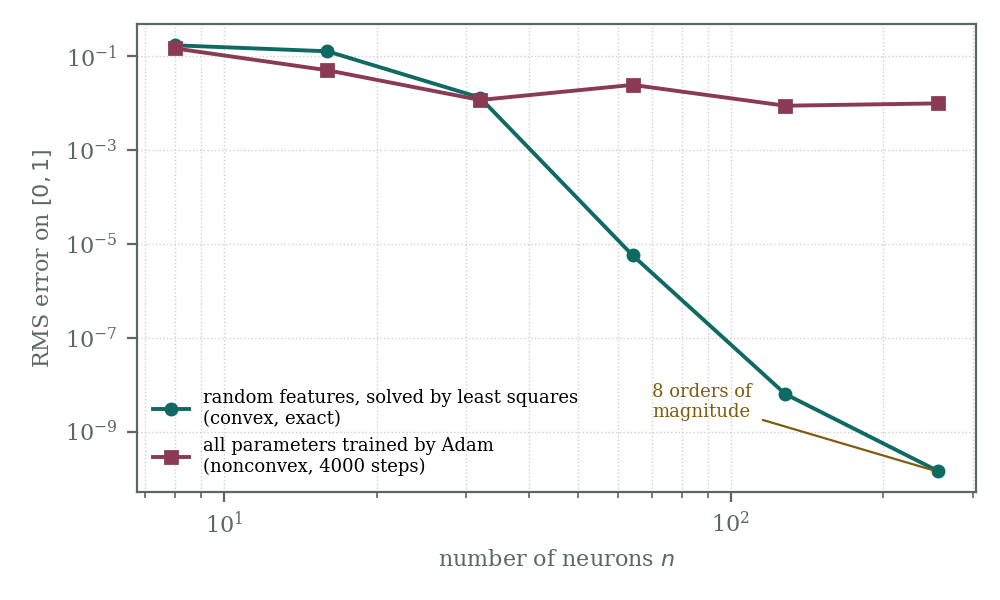
\includegraphics[width=0.78\textwidth]{figures/fig_app_vs_opt.png}
\vspace{-6pt}
\caption*{\small\color{coursgrey} Task \ref{task:gap}: medians over several seeds. The two curves
describe the same class $\Sigma_n(\tanh)$. Up to $n \approx 32$ training wins, as it should, since
it may move the neurons. Beyond, the convex solve descends to $10^{-10}$ while training stops at
$10^{-2}$.}
\end{figure}

% ================================================================
\section{Task 5 --- A finite-dimensional shadow of ``discriminatory''}

\begin{plainbox}
\textbf{The translation.} Definition 1 of the problem class says: $\sigma$ is discriminatory on $K$
when the only finite signed measure $\mu$ with $\int_K \sigma(wx+b)\,\dd\mu = 0$ for \emph{all}
$(w,b)$ is $\mu = 0$. Replace $K$ by $M$ sample points and $\mu$ by a weight vector
$\mu \in \R^M$. With $A_{ij} := \sigma(w_j x_i + b_j)$ the condition reads $A^{\!\top}\mu = 0$, so
\[
\text{``$\sigma$ is discriminatory''}
\quad\rightsquigarrow\quad
\text{$A$ has full row rank $M$, once enough features are drawn.}
\]
\end{plainbox}

\begin{task}[Rank saturation]\label{task:rank} \tagextra
Take $M = 40$ equally spaced points of $[-1,1]$.
\begin{enumerate}[label=\textbf{\arabic*.}]
\item For $\sigma = \tanh$ and for $\sigma(t) = t^2$, draw $n$ random pairs $(w_j,b_j)$ and compute
the numerical rank of $A$, for $n = 2, 5, 10, 20, 40, 100, 400$. \emph{Predict the saturation value
for $t^2$ before running}, and justify it with a number you already know.
\item Interpret the orthogonal complement of the row space in the $t^2$ case. What object, in the
language of Definition 1, does a vector of that complement represent?
\item The $\tanh$ row reaches full rank only slowly --- rank $25$ at $n = 40$, $37$ at $n=100$. The
mathematics says $A$ has full rank for generic $(w,b)$ as soon as $n \ge M$. Reconcile the two, and
name the numerical phenomenon responsible. \emph{You have just met, as a side effect, the obstacle
that Session 6 will blame for most PINN failures.}
\item \textbf{A question of logic, and the most important item of this task.} Does full row rank on
a finite point set \emph{prove} that $\sigma$ is discriminatory on $K$? Answer precisely, and say
what the experiment does and does not establish.
\end{enumerate}
\end{task}

\begin{figure}[h]
\centering
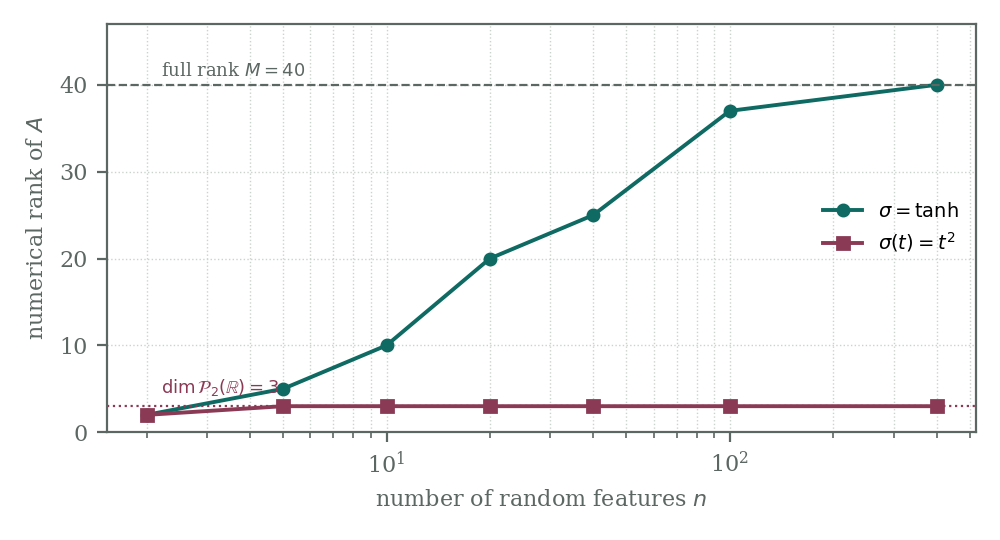
\includegraphics[width=0.72\textwidth]{figures/fig_rank.png}
\vspace{-6pt}
\caption*{\small\color{coursgrey} Task \ref{task:rank}: the quadratic activation saturates at
$3 = \dim\Pp_2(\R)$ for ever. The $37$-dimensional complement is a whole family of nonzero weight
vectors annihilating the entire class --- what \emph{not} being discriminatory looks like.}
\end{figure}

% ================================================================

\ifsolutions
\newpage
\section{Expected results, and what to say about them}
\addcontentsline{toc}{section}{Expected results}

\noindent
{\small Values obtained with the seeds fixed in the notebook; last digits vary with the sample.}

\medskip
\begin{center}
\small
\begin{tabular}{@{}llll@{}}
\toprule
\textbf{Task} & \textbf{Quantity} & \textbf{Observed} & \textbf{Statement confirmed} \\
\midrule
1 & angular spread, single ridge & $0.000\mathrm{e}{+}00$ & Prop.~1.5, first half \\
1 & angular spread, half-sum     & $\approx 1.43$ rad     & Prop.~1.5, contradiction \\[3pt]
2 & residual, degree $2^{L-1}$   & $\sim 10^{-15}$        & Ex.~2, item 5 \\
2 & residual, degree $2^{L-1}-1$ & $10^{-1}, 10^{-2}, 10^{-3}$ & bound is attained \\[3pt]
3 & $J$ at the midpoint          & $0.238577$             & $= \tfrac12\int_{-1}^1\tanh^2$ \\[3pt]
4 & frozen features, $n=256$     & $1.4\cdot10^{-10}$     & a good network exists \\
4 & all trained, $n=256$         & $9.9\cdot10^{-3}$      & gradient descent does not find it \\[3pt]
5 & rank, $\tanh$                & $2,5,10,20,25,37,40$   & discriminatory (shadow of) \\
5 & rank, $t^2$                  & $2,3,3,3,3,3,3$        & $\dim\Pp_2(\R) = 3$ \\
\bottomrule
\end{tabular}
\end{center}

\medskip

\begin{warnbox}
\textbf{The line to hold in the closing discussion.} Four of these five experiments confirm
something you proved. They are useful, but they are illustrations.

\smallskip
Task \ref{task:gap} is of a different nature: \emph{it establishes something no theorem of this
session addresses.} At $n = 256$ we exhibited an element of $\Sigma_n(\tanh)$ with error
$1.4\cdot10^{-10}$ --- so one exists, constructively, with a certificate. Adam, over the same class
and starting from the same distribution, returned $9.9\cdot10^{-3}$: eight orders of magnitude away.

\smallskip
Cybenko's theorem is silent here, and so is Barron's: both bound $\Ee_{\mathrm{app}}$, and what we
have just measured is $\Ee_{\mathrm{opt}}$. Session 4 will give that decomposition its name, and
Session 6 will spend ninety minutes on the term we have just met. If a single number from this lab
is to survive until then, it is the ratio $10^{-10}$ against $10^{-2}$.
\end{warnbox}

\medskip
\noindent
\textbf{Two traps worth anticipating.}

\smallskip\noindent
\emph{``The experiment is unfair, you did not tune the optimiser.''} Correct, and item 6 of Task
\ref{task:gap} invites exactly that objection. Let students run it. A longer budget, a learning-rate
schedule or L-BFGS improves the red curve, and does not close a gap of eight orders of magnitude.
The honest conclusion is not ``gradient descent is bad'' but ``on this class, the convex problem is
solved without effort and the nonconvex one requires care, luck and a stopping rule'' --- which is
precisely the claim the course will make again in Session 6, with theory.

\smallskip\noindent
\emph{``Frozen random features are not really a network.''} They are: a frozen-feature model is an
element of $\Sigma_n(\sigma)$ with its $(w_i,b_i)$ chosen before the data are seen. It is a
\emph{restricted} search, which is why it is a legitimate \emph{upper} bound on the best error over
$\Sigma_n(\sigma)$, and why the comparison in Task \ref{task:gap} is conservative rather than rigged:
the nonconvex method is losing to a handicapped opponent.

% ================================================================
\fi

\section*{Files}
\addcontentsline{toc}{section}{Files}

\begin{itemize}[leftmargin=*, itemsep=3pt]
\item \code{lab1-student.ipynb} --- the lab, with the five tasks and the gaps to fill.
\item \code{lab1-solutions.ipynb} --- the same notebook, complete, with the commentary that belongs
to each result. It runs end to end in about three minutes on a laptop with no GPU.
\end{itemize}

\vspace{4pt}
\noindent
{\small Requirements: \code{torch}, \code{numpy}, \code{matplotlib}. Double precision is set at the
top of the notebook with \code{torch.set\_default\_dtype(torch.float64)} and this matters: Tasks
\ref{task:poly} and \ref{task:gap} measure errors below $10^{-8}$, which single precision cannot
represent. Session 2 explains why that threshold is where it is.}

\end{document}
